\documentclass[a4paper,10pt]{article}
\usepackage{Sweave}
\begin{document}
\Sconcordance{concordance:PreReport.tex:PreReport.Rnw:%
1 7 1 1 0 7 1 1 5 10 1 1 6 1 0 4 1 3 0 1 2 10 1 1 2 16 0 1 2 1 4 3 1 1 %
10 2 0 1 2 4 0 1 5 9 1 1 6 1 0 3 1 3 0 1 5 29 1 1 5 1 3 2 0 2 1 5 0 1 1 %
5 0 1 1 5 0 1 1 6 0 1 2 1 4 15 1 1 7 1 0 3 1 1 2 4 0 1 2 10 1 1 2 1 0 1 %
1 1 2 6 0 1 2 6 0 1 2 13 0 1 5 7 1 1 2 1 0 3 1 6 0 1 2 4 1 1 2 1 0 1 1 %
5 0 1 1 6 0 1 2 1 1 1 2 1 0 1 1 1 2 1 0 1 1 6 0 1 2 1 1 1 70 27 1 1 6 1 %
4 3 0 1 1 3 0 1 2 1 4 15 1 11 0 1 10 3 1 11 0 1 10 2 1 24 0 1 23 7 1 1 %
6 1 7 1 4 9 1 1 6 1 9 1 4 13 1 1 7 1 0 1 1 1 7 6 0 1 1 1 2 1 1 5 0 1 1 %
5 0 1 1 5 0 1 1 6 0 1 5 11 1 12 0 1 11 5 1 14 0 1 13 17 1 14 0 1 13 5 1 %
1 6 1 0 5 1 3 0 1 5 8 1 1 2 20 0 1 18 30 1 1 7 2 0 4 1 5 0 1 1 6 0 1 5 %
11 1 1 2 1 0 3 1 1 2 1 0 3 1 4 0 1 3 11 1 1 3 2 0 1 2 1 0 1 3 2 0 1 2 4 %
0 1 2 2 1 1 3 2 0 1 1 1 2 1 0 1 2 1 0 1 1 3 0 1 2 35 1}


\section{Introduction}
\subsection{Background}
The core graphics system in R can been divided in to two main packages. The first package is the graphics package. It is older and it provides the original GRZ graphics system from S, sometimes referred to as ``traditional'' graphics. It is relatively fast and many other R packages build on top of it. The newer package is the grid package. It is actually slower but is has more flexibility and additional features compared to the graphics package. \\\\
A graph that is drawn using grid can been edited in many more ways than a graph that has been drawn using the basic graphics package. However, there is a new package, called gridGrahics, which allows us to convert a plot that has been drawn by the graphics package to an equivalent plot drawn by grid graphics. This means that the additional flexibility and features of grid become available for any plot drawn using the graphics package. \\\\

\subsection{The \texttt{gridGraphic} package}
\texttt{gridGraphic} is like a 'translator' that translate the plot which been drawn by using the basic graphics package to the plot which been drawn by using grid package. 
The \texttt{gridGraphic} package has a main function called \textt{grid.echo()}, which takes a recorded plot (or NULL for the current plot of the current graphic dervice) as an argument. Then it replicate the 
plot by using grid so that the user may edites the plot in more way than the plot drawn by bacis graphic package.
The following code provides a quick example. We generate 25 random numbers for x and y. First, we draw a scatter plot using the function plot() from the basic graphic package, then we redraw it using grid.echo() from the gridGraphic package with grid.
\begin{Schunk}
\begin{Sinput}
> setwd(110)
> x = runif(25)
> y = runif(25)
> plot(x,y, pch = 16)
> grid.echo()
\end{Sinput}
\end{Schunk}
\begin{figure}[H]
\begin{center}
  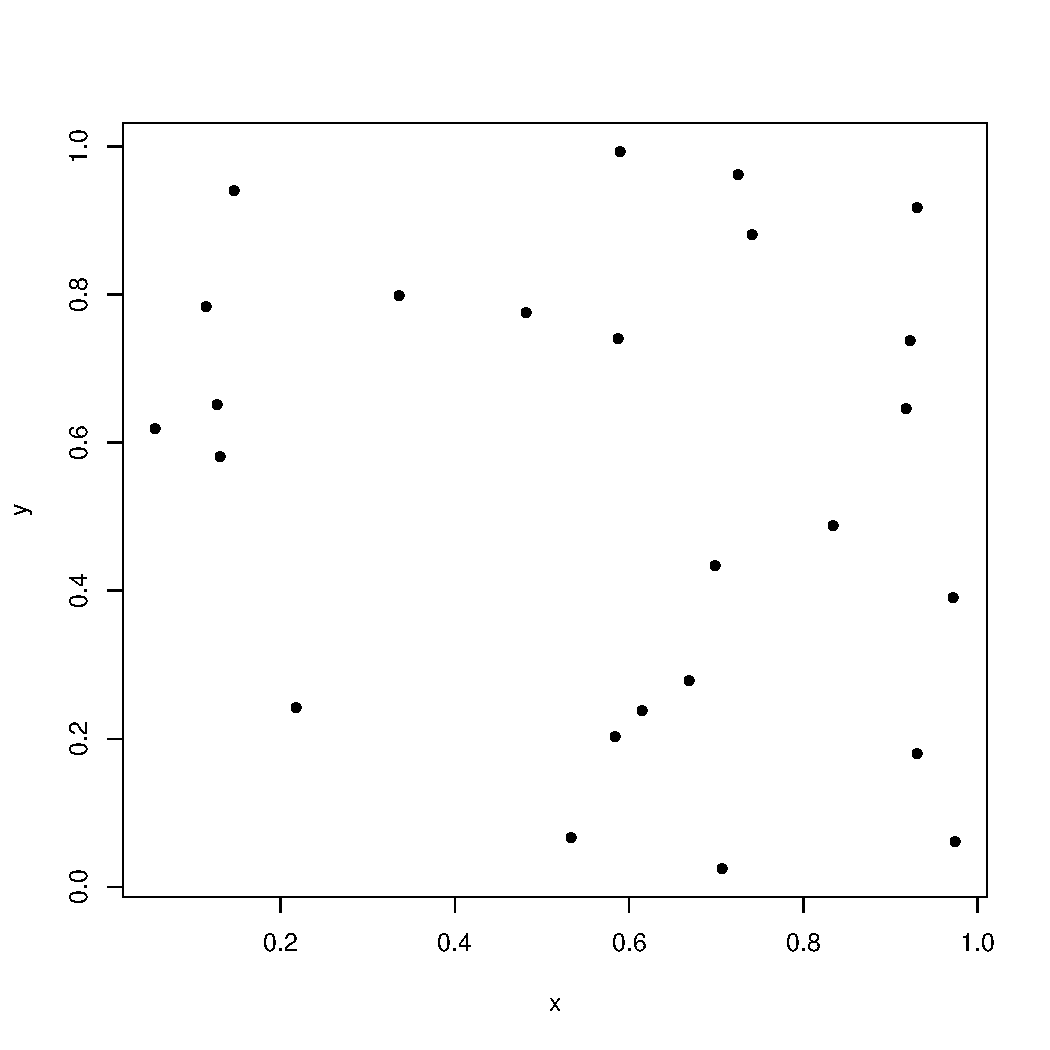
\includegraphics[height = 5cm, width = 6cm]{figure/basic.pdf}
  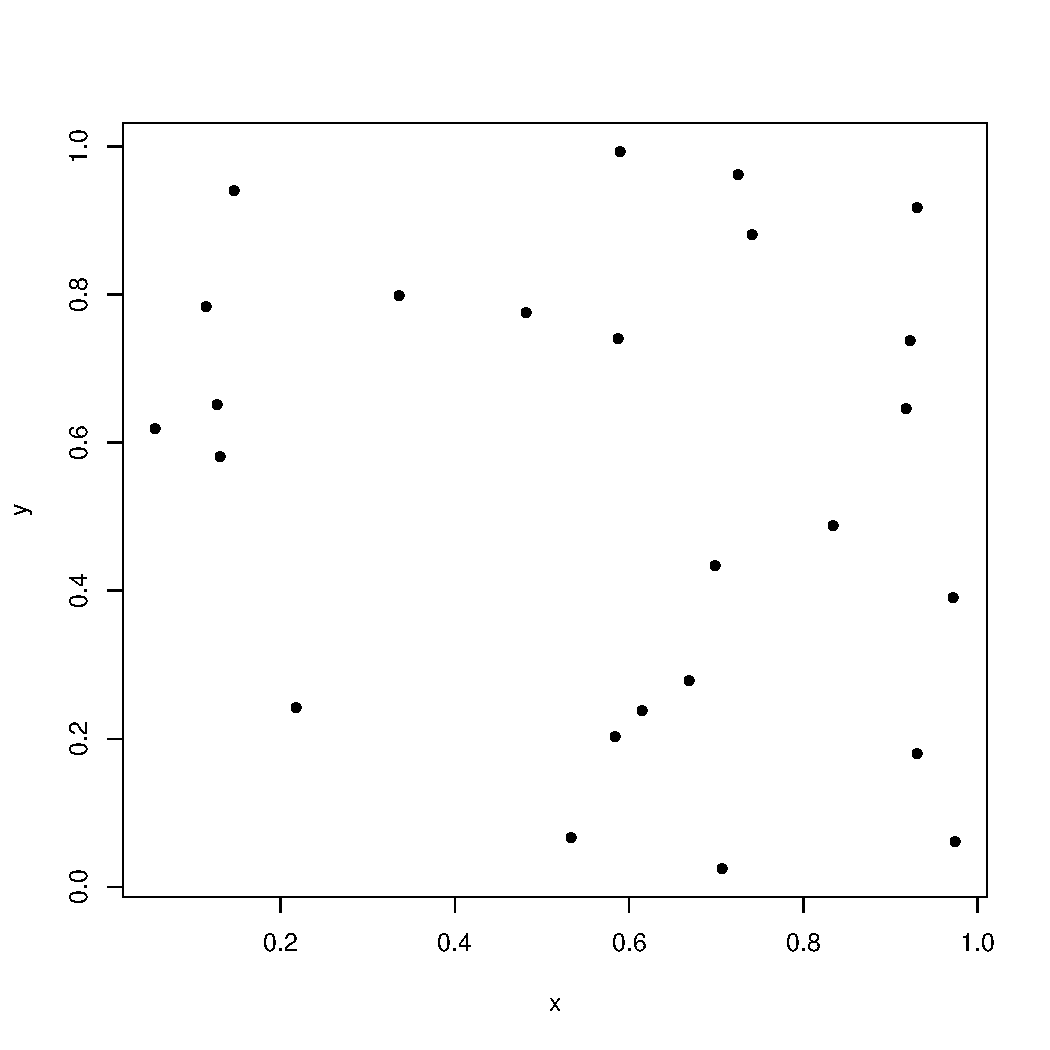
\includegraphics[height = 5cm, width = 6cm]{figure/echo.pdf}
  \caption{The left plot drawn by using plot(), the Right plot is redraw it by using grid.echo() on grid graphic system, overall, they are identical to each other}
  	\label{figure1}
\end{center}
\end{figure}


Alternatively, one example that shows the advantage of drawing the plot using grid rather than basic is that there is an object, called grid grobs, which recored a list of the details of each components of the plot that been drawn. The list of grobs can been seen by calling the function \texttt{grid.ls()}. \\\\

\begin{Schunk}
\begin{Sinput}
> graphics-background
> graphics-plot-1-points-1
> graphics-plot-1-bottom-axis-line-1
> graphics-plot-1-bottom-axis-ticks-1
> graphics-plot-1-bottom-axis-labels-1
> graphics-plot-1-left-axis-line-1
> graphics-plot-1-left-axis-ticks-1
> graphics-plot-1-left-axis-labels-1
> graphics-plot-1-box-1
> graphics-plot-1-xlab-1
> graphics-plot-1-ylab-1
\end{Sinput}
\end{Schunk}

As we see, the \texttt{grid.ls()} returns a list of grid grobs of the pervious plot that been redrawn by grid. there is one element called "graphics-plot-1-bottom-axis-labels-1" which is the element of the label of the bottom axis. There are several function on the \texttt{grid} package that used for mainpulate this grob. For example, if the user wants to rotate the labels of the bottom axis by 30 degrees and changes the color from default to orange, then the following code mainpulate this changes.

\begin{Schunk}
\begin{Sinput}
> grid.edit("graphics-plot-1-bottom-axis-labels-1", 
+           rot=30, gp=gpar(col="orange"))
\end{Sinput}
\end{Schunk}

\begin{figure}[H]
\begin{center}
  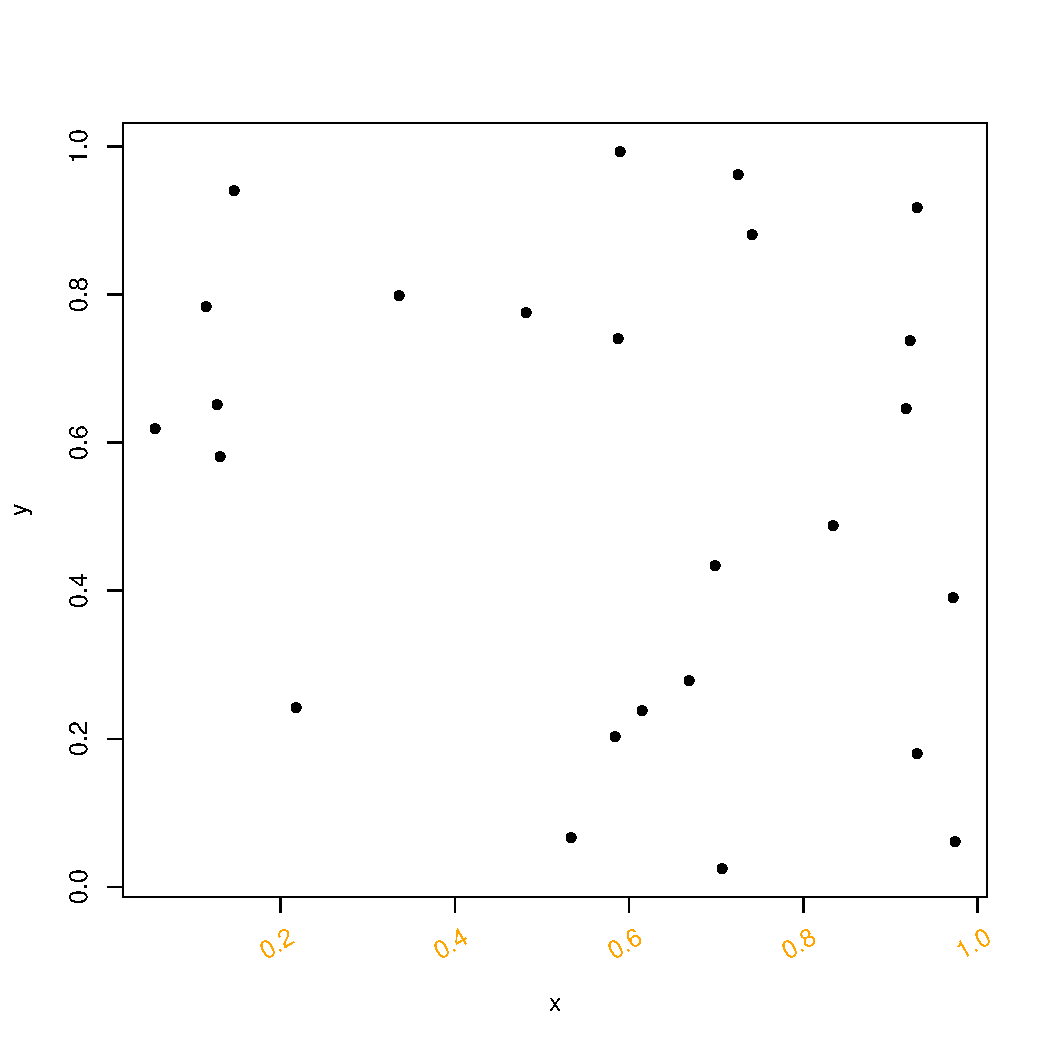
\includegraphics[height = 5cm, width = 6cm]{figure/gridedit.pdf}
  \caption{The angel and the color of the bottom axis of the previous plot been change by 30 degree and orange}
  	\label{figure3}
\end{center}
\end{figure}





\subsection{The problem}
The grid.echo() function can replicate most plots that are drawn by the graphics package. However, there are a few functions in the graphics package that grid.echo() cannot replicate. One such function is persp() which draws 3-dimemtional surfaces, the other one is the filled.contour(). This leads to the aim of this project. If we can draw a plot with persp() or filled.countour(), the result from calling grid.echo() is a blank screen 

\begin{Schunk}
\begin{Sinput}
> x <- y <- seq(-4*pi, 4*pi, len = 27)
> r <- sqrt(outer(x^2, y^2, "+"))
> filled.contour(cos(r^2)*exp(-r/(2*pi)), frame.plot = FALSE, plot.axes = {})
\end{Sinput}
\end{Schunk}

\begin{figure}[H]
\begin{center}
  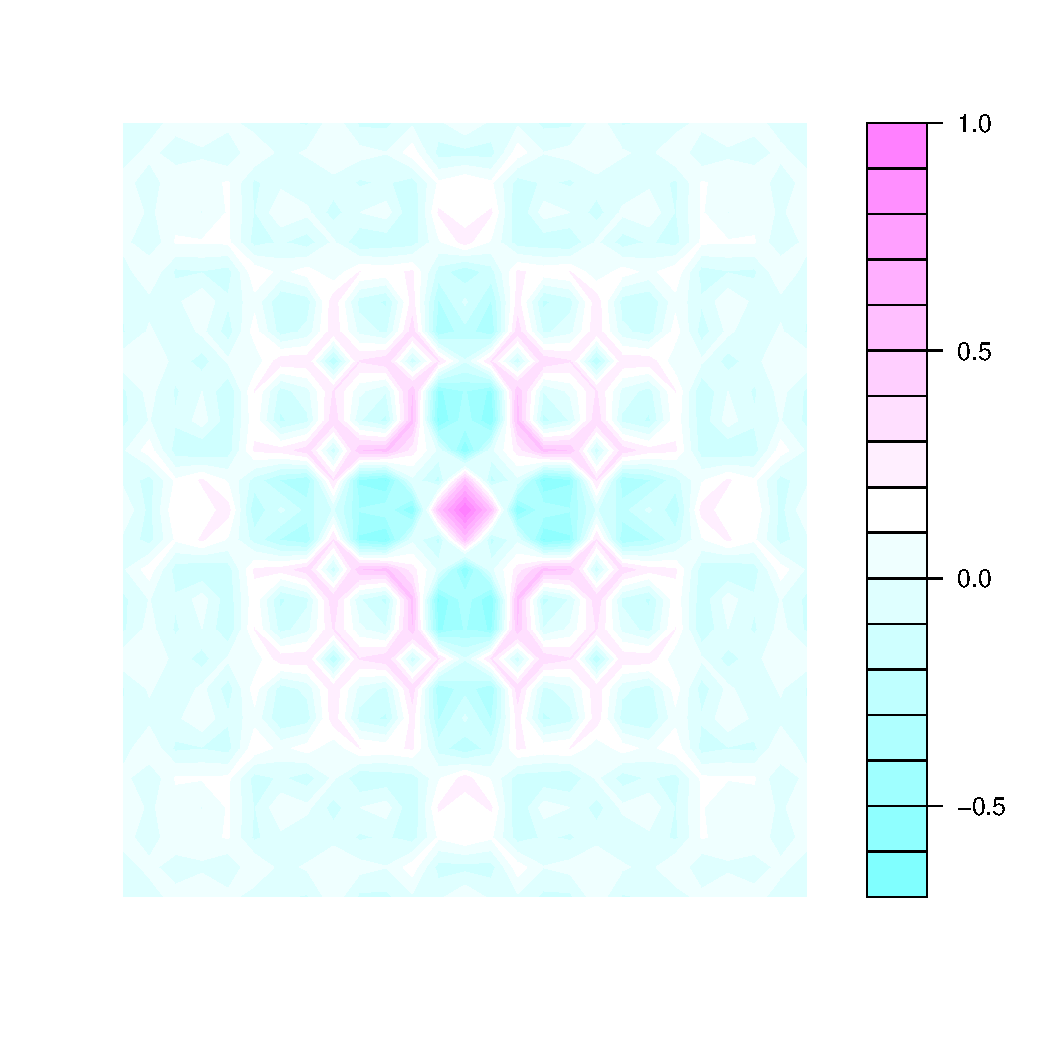
\includegraphics[height = 5cm, width = 6cm]{figure/filled-contour.pdf}
  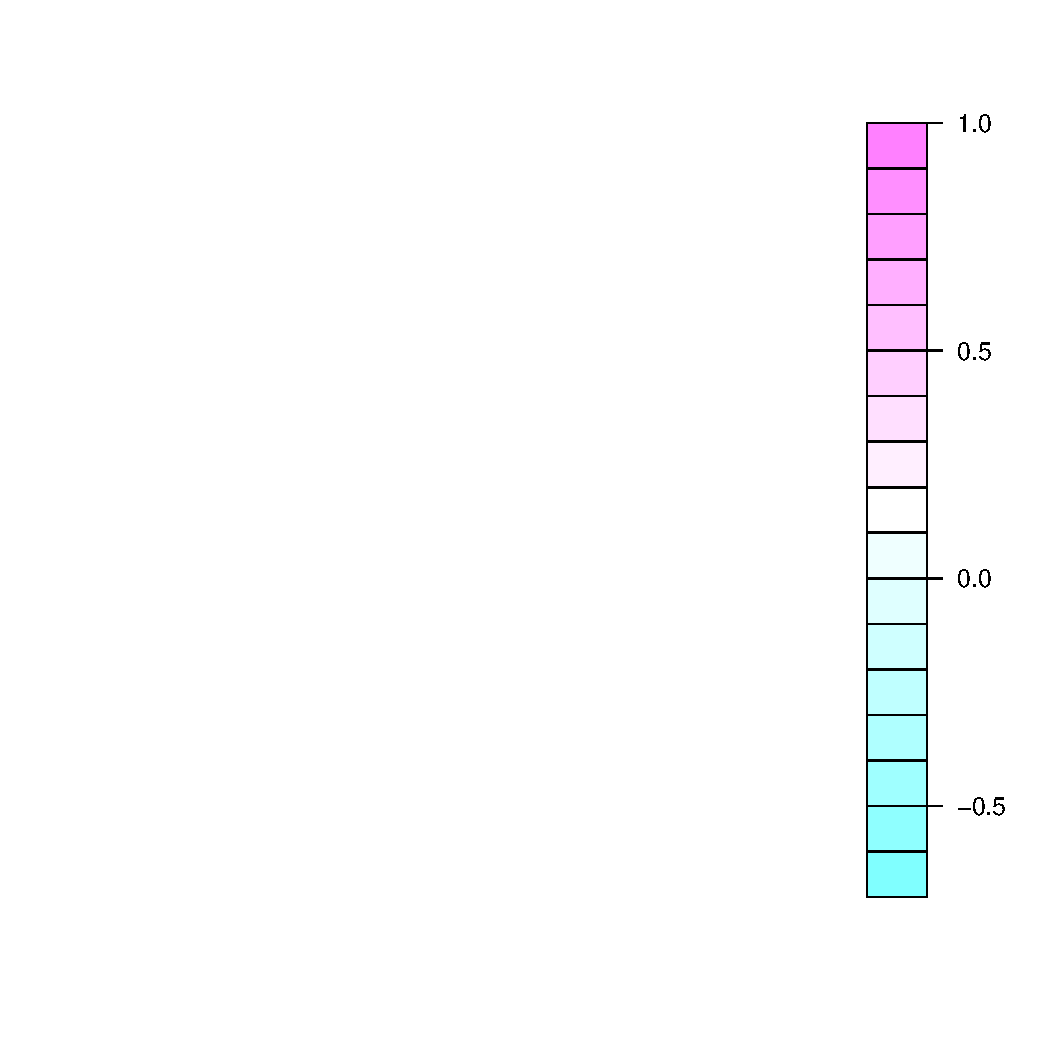
\includegraphics[height = 5cm, width = 6cm]{figure/filled-contour-gridecho.pdf}
  \caption{The angel and the color of the bottom axis of the previous plot been change by 30 degree and orange}
  	\label{figure3}
\end{center}
\end{figure}


NOTE to Jason: explain how gridGraphics works first: graphics display list; gridGraphics implements an R version of each low-level C function on the display list (e.g., for C\_plot\_xy there is an R function called C\_plot\_xy in the gridGraphics package). THEN maybe write about 3D to 2D transformations, but only maybe.

Firstable, it is necessary to understand some important theory behind the 3-dimentional plot, such as the transformation from 3-D to 2-D, the drawing order of each ploygons (will be explained later). ect. Then we try to redraw it by using the grid package and we can replicate this function on grid by using the grid.echo().


\begin{figure}[h]
  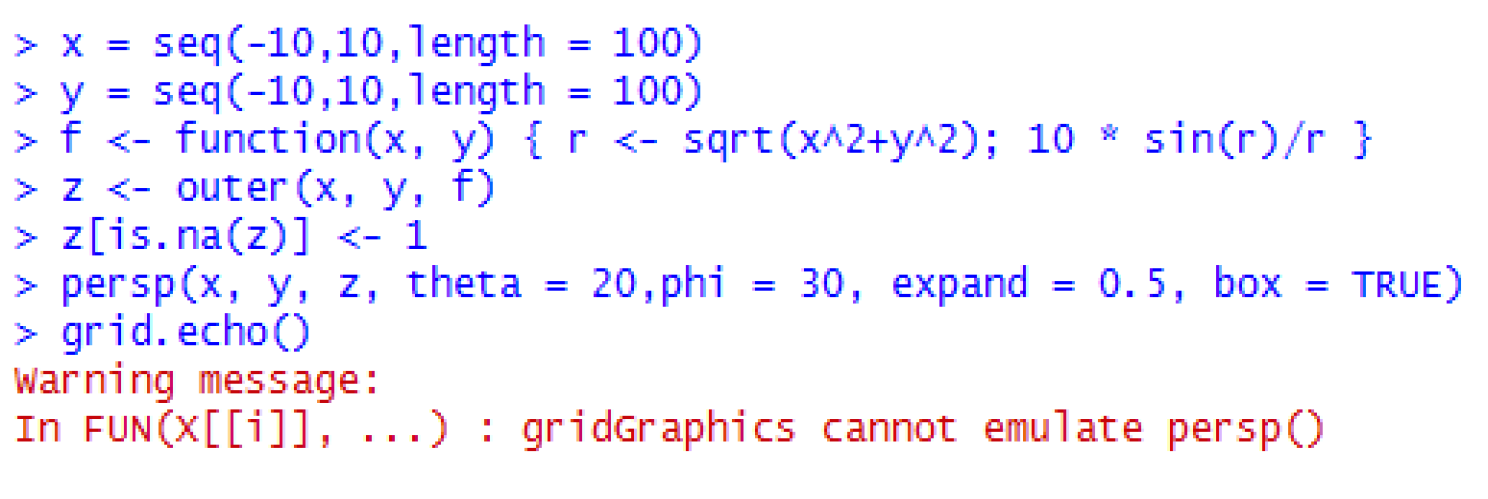
\includegraphics[height = 2.5cm, width = 8.5cm]{figure/warning.png}
  \caption{an example shows that the grid.echo() cannot replicate the persp() on grid}
  	\label{figure2}
\end{figure}

\end{document}
